\section{Citizens}
	\subsection{Registration}
	If you want to create a personal account for \textit{Soldino}, visit the
	homepage, make sure you are logged in your MetaMask\glosp account
	and then check that the switch button is set on "Citizen".\\
	\begin{figure}[H]
		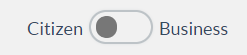
\includegraphics[width=5cm]{res/images/user_citizen.png}
		\centering
		\caption{Select "Citizen" from the switch button}
	\end{figure}	
	\noindent Then, insert your data in the form. 
	\begin{figure}[H]
		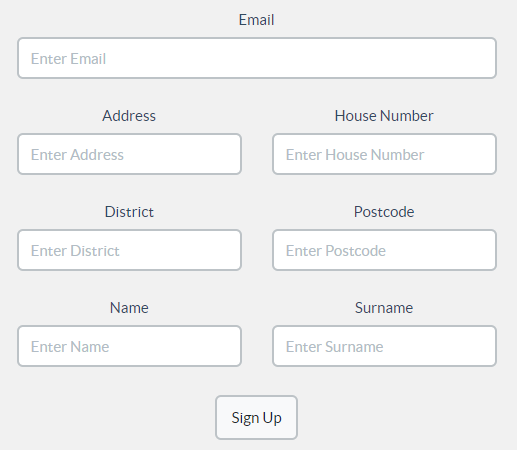
\includegraphics[width=10cm]{res/images/citizen_signup.png}
		\centering
		\caption{Citizen signup form}
	\end{figure}
	\noindent After you have completed all the
	fields with your informations, press the "Sign up" button. If an entry 
	is not valid (e.g. the email address does not contain a valid domain), 
	the system will let you know it and you have to edit that field to continue.
	If all informations are correct, a pop-up window will ask you 
	to give \textit{Soldino} access to your information.\\
	\begin{figure}[H]
		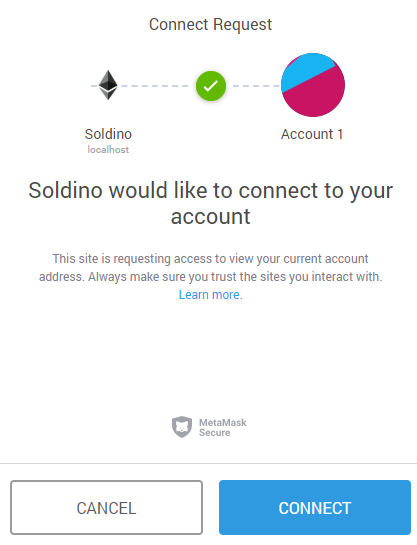
\includegraphics[width=10cm]{res/images/metamask_connect.png}
		\centering
		\caption{Connecting MetaMask to \textit{Soldino}}
	\end{figure}
	\noindent Press "Connect" and you will be redirected to a page 
	congratulating you for your registration on the platform.
	\begin{figure}[H]
		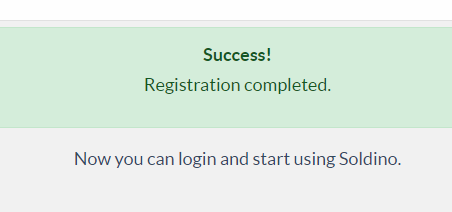
\includegraphics[width=10cm]{res/images/registration_complete.png}
		\centering
		\caption{Completed registration message}
	\end{figure}
		\subsubsection{Citizen is already registered}
		If your Ethereum\glosp address is already registered in the platform, you will 
		see an error message.
		\begin{figure}[H]
			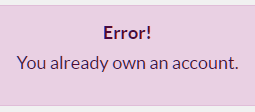
\includegraphics[width=10cm]{res/images/user_already_registered.png}
			\centering
			\caption{Error message if the user is already registered}
		\end{figure}
		\noindent Just press "Login" to log in your personal account.
	\subsection{Login}
	If you already have a personal account, press the "login" button on the 
	top right of the homepage, you will be automatically logged in your account 
	(there is no need for a username or password, all data are done via MetaMask). 
	\\You must are logged in your MetaMask\glo{} account and then you can be logged on \textit{Soldino}.
		\subsubsection{Account is disabled}
		If your account was disabled by the Government, you will see an error 
		message.
		\begin{figure}[H]
			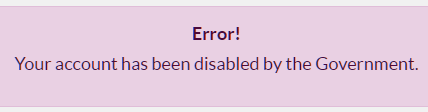
\includegraphics[width=10cm]{res/images/user_disabled.png}
			\centering
			\caption{Error shown if your account has been disabled by the Government}
		\end{figure}
	\noindent If your account is disabled, you cannot access it any more until it 
	is enabled again by the Government.
	\subsection{Logout}
	To log out of \textit{Soldino}, you just have to log out of 
	MetaMask\glo{}. First you have to press MetaMask's icon on the top 
	right of the browser, press your account's icon and then press "Log out"
	on the top right.
	\begin{figure}[H]
		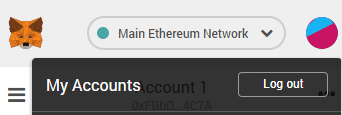
\includegraphics[width=10cm]{res/images/logout_metamask.png}
		\centering
		\caption{Logging out}
	\end{figure}
	\subsection{Buying}
	Note that all prices shown in the platform are in Cubits\glosp, 
	\textit{Soldino}'s own special token. Also, note that 1 Cubit equals 1 Euro.
		\subsubsection{Searching}
		You can search for products by name using the search bar that can be 
		found on the top of the page. After you start typing you will see 
		all results that match your search. If no matching products are found 
		you will get an error message showing you that.
%		
		\subsubsection{Cart}
		You can add products in your cart, after selecting the quantity you 
		need, by pressing the "Add to cart" button under it.
		\begin{figure}[H]
			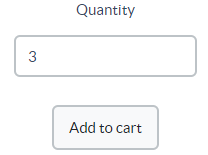
\includegraphics[width=7cm]{res/images/add_to_cart.png}
			\centering
			\caption{Adding a product to your cart}
		\end{figure}
		\noindent The cart's number shows you how many unique products 
		are in it. You can access your cart by pressing the shopping cart icon 
		in the navigation bar at the top of the page.
		\begin{figure}[H]
			
\includegraphics[width=3cm]{res/images/cart_icon.png}
			\centering
			\caption{Icon to access your cart}
		\end{figure}
		\noindent Here you will see the total for your order and you will find 
		every item you have previously selected with their quantity. If you 
		need to modify the quantity press the "+" or "-" buttons.
		\begin{figure}[H]
			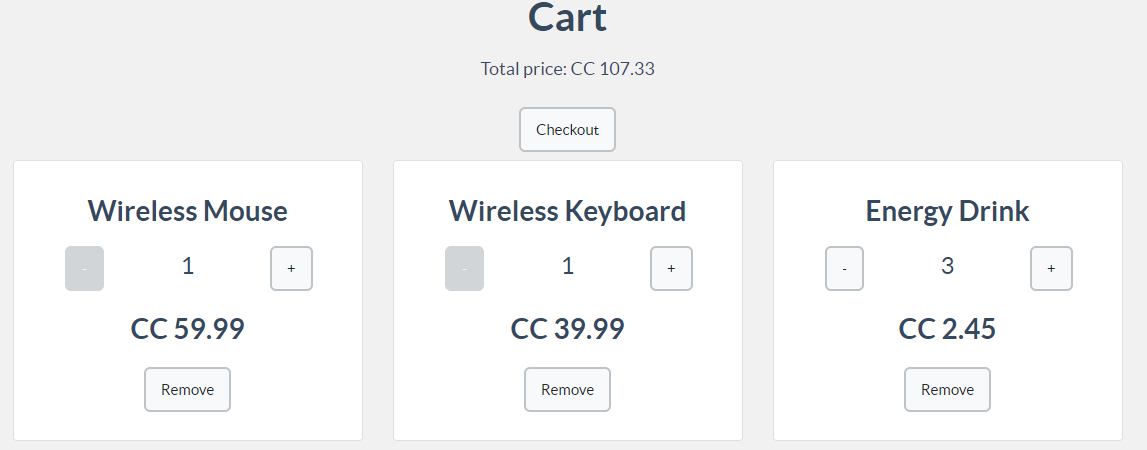
\includegraphics[width=15cm]{res/images/cart_example.png}
			\centering
			\caption{Example of a cart's content}
		\end{figure}
		\noindent When you want to proceed with the order, press the "Checkout" 
		button, in this way you will be redirected to the checkout page.
	\subsubsection{Checkout}
	In the checkout page you will be able to choose where your products will be 
	delivered to by using the radio buttons: you can either select the address 
	you gave during registration or enter a new one.\\
	\begin{figure}[H]
		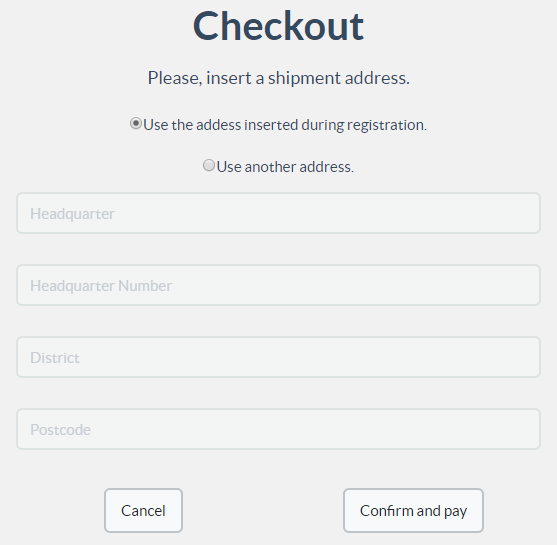
\includegraphics[width=10cm]{res/images/checkout.png}
		\centering
		\caption{Example of a checkout page}
	\end{figure}
	\noindent Press the "Confirm and pay" button to proceed. In a new 
	pop up window MetaMask\glosp will ask you to confirm the transaction. The price 
	shown here will be a little higher because it includes the Gas fee. \\
	Press "Cancel" button if you do not want to continue, you will be redirected to your cart.
	\subsubsection{Past orders}
	You can visit the page containing all past orders by pressing the "Orders" 
	button in the navigation bar at the top of the page.
%
	Here you will find a chronology list of every purchase that you made through 
	\textit{Soldino}. Each order shows when it was made, who was the seller, 
	what were the items bought, where it was shipped to and how much you paid for it.
	\begin{figure}[H]
		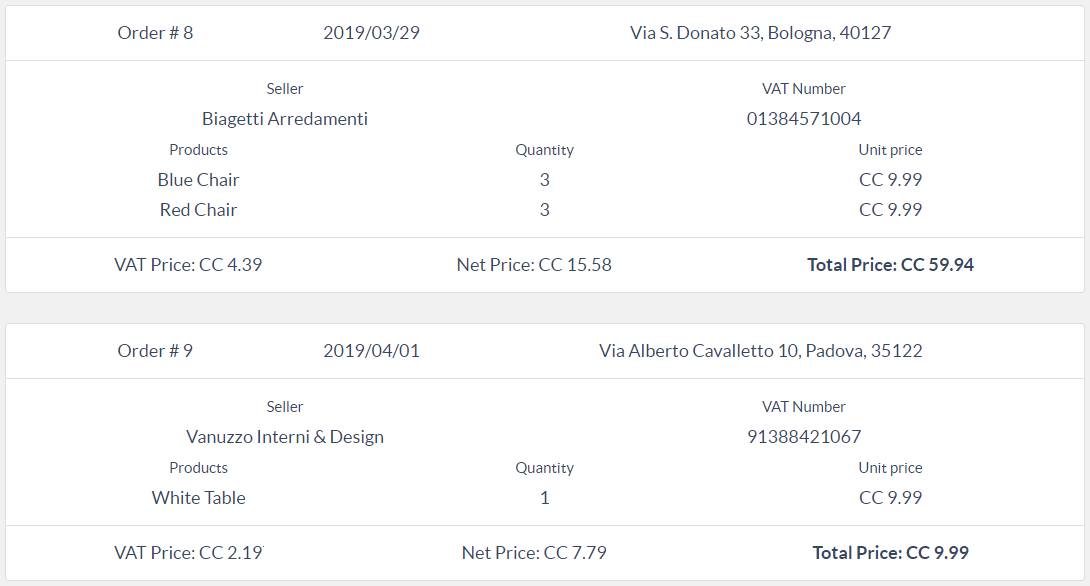
\includegraphics[width=15cm]{res/images/past_orders.png}
		\centering
		\caption{Example of past orders}
	\end{figure}